\documentclass[../../../../main.tex]{subfiles}

\begin{document}

\section*{第1問}

\begin{proof}[解]
\begin{enumerate}
  \item[(1)] $x=\dfrac{c}{b},\ y=\dfrac{d}{a}$とおける。ただし，$a,b,c,d\in\mathbb{N}$，$b$と$c$，$a$と$d$は互いに素，又対称性から$x>y$とする。 $\cdots$①
  \[
  \frac{1}{|x-y|}=\frac{1}{x-y}=\frac{ab}{ac-bd} \quad(\because①)
  \]
  \[
  f(x)+f(y)=b^2+a^2
  \]
  から
  \[
  f(x)+f(y)-\frac{2}{|x-y|}=a^2+b^2-\frac{2ab}{ac-bd}
  \]
  \[
  =(a-b)^2+2ab\left(1-\frac{1}{ac-bd}\right)\ge0
  \]
  となり示された。（$ac-bd\in\mathbb{N}$から，$\dfrac{1}{ac-bd}\le1$）

  \item[(2)] $x_n=\dfrac{2}{3n+4}$とおく。$k\in\mathbb{N}$とする。
  \[
  n=2k\text{の時，}x_n=\frac{1}{3k+2}, \qquad n=2k-1\text{の時，}x_n=\frac{2}{6k+1}
  \]
  であるから，$F_n=\{f(x_n)+f(x_{n+1})\}|x_n-x_{n+1}|$とおくと，$n\to\infty$で$k\to\infty$で，
  \[
  F_{2k}=\left|\frac{1}{3k+2}-\frac{2}{6k+7}\right|\left\{(3k+2)^2+(6k+7)^2\right\}
  \]
  \[
  =\frac{3\left\{(3k+2)^2+(6k+7)^2\right\}}{(3k+2)(6k+7)}
  =\frac{3\left\{(3+2/k)^2+(6+7/k)^2\right\}}{(3+2/k)(6+7/k)}\longrightarrow\frac{3\cdot45}{18}=\frac{15}{2}\quad(k\to\infty)
  \]
  \[
  F_{2k-1}=\left|\frac{2}{6k+1}-\frac{1}{3k+2}\right|\left\{(3k+2)^2+(6k+1)^2\right\}
  \]
  \[
  =\frac{3\left[(3+2/k)^2+(6+1/k)^2\right]}{(6+1/k)(3+2/k)}\longrightarrow\frac{15}{2}\quad(k\to\infty)
  \]
  以上から
  \[
  (\text{与式})=\frac{15}{2}
  \]
\end{enumerate}
\end{proof}

\newpage

\section*{第2問}

\begin{proof}[解]
$0<t\le\dfrac12\ \cdots$①，$y=f(t)=\dfrac12\left\{t+\dfrac{x(2-x)}{t}\right\}$とおく。
\[
f'(t)=\frac12\left\{1+\frac{x(x-2)}{t^2}\right\}
\]
であり，以下のようになる。

\textbf{$1^\circ$ $x\le0,\ 2\le x$の時}

$f'(t)>0$から，$\displaystyle\lim_{t\to0}f(t)<y\le f\left(\frac12\right)$

\textbf{$2^\circ$ $0<x<1-\dfrac{\sqrt3}{2},\ 1+\dfrac{\sqrt3}{2}<x<2$の時}

下表を得る。
\begin{center}
\begin{tabular}{c|ccccc}
$t$ & $0$ & & $\sqrt{x(2-x)}$ & & $\frac12$ \\
\hline
$f'$ & & $-$ & $0$ & $+$ & \\
\hline
$f$ & & $\searrow$ & & $\nearrow$ &
\end{tabular}
\end{center}
したがって，$\displaystyle\lim_{t\to0}f(t)>f\left(\frac12\right)$から
\[
f(\sqrt{x(2-x)})\le f(t)<\lim_{t\to0}f(t)
\]

\textbf{$3^\circ$ $1-\dfrac{\sqrt3}{2}\le x\le1+\dfrac{\sqrt3}{2}$の時}

$f'(t)<0$から $\displaystyle f\left(\frac12\right)\le y<\lim_{t\to0}f(t)$

ここで
\[
f\left(\frac12\right)=-x^2+2x+\frac14=-(x-1)^2+\frac54, \qquad f(\sqrt{x(2-x)})=\sqrt{x(2-x)}
\]
図示して，下図斜線部（境界は$x=0,2$を除く）。

\begin{center}
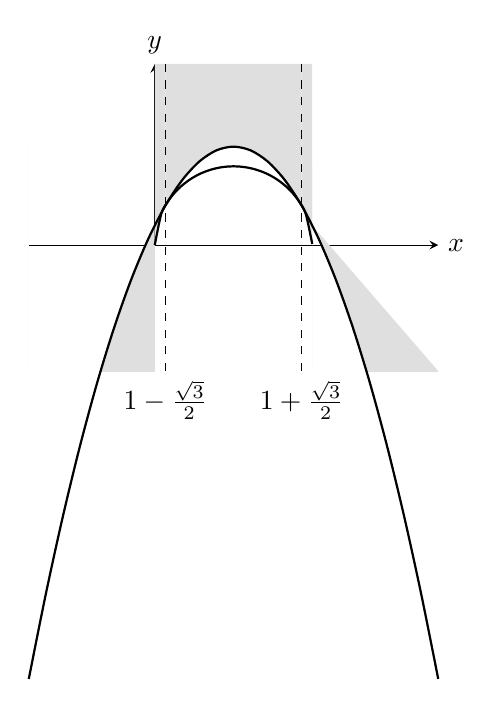
\begin{tikzpicture}[scale=1.0, >=stealth]
  \draw[->] (-1.6,0) -- (3.6,0) node[right] {$x$};
  \draw[->] (0,-1.6) -- (0,2.3) node[above] {$y$};
  \begin{scope}
    \clip (0,0) rectangle (0.134,2.3);
    \fill[gray!25] plot[domain=0:0.134,samples=20] (\x,{sqrt(\x*(2-\x))}) -- (0.134,2.3) -- (0,2.3) -- cycle;
  \end{scope}
  \begin{scope}
    \clip (0.134,0) rectangle (1.866,2.3);
    \fill[gray!25] plot[domain=0.134:1.866,samples=40] (\x,{-(\x-1)*(\x-1)+1.25}) -- (1.866,2.3) -- (0.134,2.3) -- cycle;
  \end{scope}
  \begin{scope}
    \clip (1.866,0) rectangle (2,2.3);
    \fill[gray!25] plot[domain=1.866:2,samples=20] (\x,{sqrt(\x*(2-\x))}) -- (2,2.3) -- (1.866,2.3) -- cycle;
  \end{scope}
  \begin{scope}
    \clip (-1.6,-1.6) rectangle (0,2.3);
    \fill[gray!25] (-1.6,-1.6) -- (-1.6,1.25) plot[domain=-1.6:0,samples=20] (\x,{-(\x-1)*(\x-1)+1.25}) -- (0,-1.6) -- cycle;
  \end{scope}
  \begin{scope}
    \clip (2,-1.6) rectangle (3.6,2.3);
    \fill[gray!25] (2,-1.6) -- (2,1) plot[domain=2:3.6,samples=20] (\x,{-(\x-1)*(\x-1)+1.25}) -- (3.6,-1.6) -- cycle;
  \end{scope}
  \draw[domain=0:2, smooth, thick] plot (\x,{sqrt(\x*(2-\x))});
  \draw[domain=-1.6:3.6, smooth, thick] plot (\x,{-(\x-1)*(\x-1)+1.25});
  \draw[dashed] (0.134,-1.6) -- (0.134,2.3);
  \draw[dashed] (1.866,-1.6) -- (1.866,2.3);
  \node[below] at (0.134,-1.6) {$1-\frac{\sqrt3}{2}$};
  \node[below] at (1.866,-1.6) {$1+\frac{\sqrt3}{2}$};
\end{tikzpicture}
\end{center}
（$0<x<2$の部分は上側の曲線・放物線の下側包絡線から上方に無限に広がる領域，$x\le0,2\le x$の部分は放物線$y=-(x-1)^2+\frac54$の下方に無限に広がる領域。灰色部は図の枠内で切り取って表示している。）
\end{proof}

\newpage

\section*{第3問}

% (原稿において第3問の解答は空欄)

\newpage

\section*{第4問}

\begin{proof}[解]
$A+B+C=\pi,\ A,B,C>0\ \cdots$①
\[
F=\sin3A+\sin3B+\sin3(\pi-A-B) \quad(\because①)
\]
\[
=\sin3A+\sin3B+\sin3(A+B)
\]
対称性から$A=B$として良い。$0<A<\dfrac{\pi}{2}\ \cdots$②であり，
\[
F=2\sin3A+\sin6A
\]
\[
\frac{dF}{dA}=6\cos3A+6\cos6A \quad\cdots\text{③}
\]
$t=\cos3A$とおくと，
\[
\frac{③}{6}=2t^2+t-1=(t+1)(2t-1)
\]
下表を得る。
\begin{center}
\begin{tabular}{c|ccccc}
$A$ & $0$ & & $20^\circ$ & & $\frac{\pi}{2}$ \\
\hline
$t$ & $1$ & & $\frac12$ & & $0$ \\
\hline
$F'$ & & $+$ & $0$ & $-$ & \\
\hline
$F$ & & $\nearrow$ & & $\searrow$ &
\end{tabular}
\end{center}
$A=20^\circ$の時，$\max F=\dfrac{3\sqrt3}{2}$

$A\to0$の時，$F\to0$

$A\to\dfrac{\pi}{2}$の時，$F\to-2$

以上から
\[
\text{(1)}\quad\frac{3\sqrt3}{2} \qquad\qquad \text{(2)}\quad -2<F\le\frac{3\sqrt3}{2}
\]
\end{proof}

\newpage

\section*{第5問}

\begin{proof}[解]
\[
\ell_1: y=-x-2, \qquad \ell_2: y=-\frac{1}{t^2}x+\frac{2}{t}
\]
$\ell_1$と$y=-\dfrac3x$の交点のうち$A(1,-3)$，$\ell_2$と$y=-\dfrac3x$の交点のうち$B\left(3t,-\dfrac1t\right)$，$\ell_1$と$\ell_2$の交点$C\left(-\dfrac{2t}{t-1},\dfrac{2}{t-1}\right)$とおく。$S(t)$は，直線$AC$，$BC$と曲線$AB$（$y=-3/x$）とで囲まれた図形の面積であり，右のように分割できる。

\begin{center}
\begin{tikzpicture}[scale=0.7, >=stealth]
  \coordinate (A) at (1,-3);
  \coordinate (B) at (6,-0.5);
  \coordinate (C) at (-2,3);
  \coordinate (D) at (1,-0.5);
  \draw (C) -- (A);
  \draw (B) -- (C);
  \draw[domain=1:6,smooth] plot (\x,{-3/\x});
  \draw[dashed] (D) -- (A);
  \draw[dashed] (D) -- (B);
  \fill (A) circle (1.2pt) node[below] {$A$};
  \fill (B) circle (1.2pt) node[right] {$B$};
  \fill (C) circle (1.2pt) node[above] {$C$};
  \fill (D) circle (1.2pt) node[above right] {$D\left(1,-\frac1t\right)$};
\end{tikzpicture}
\end{center}

補助点$D\left(1,-\dfrac1t\right)$をとると，
\[
\triangle ADB=\frac12(3t-1)\left(3-\frac1t\right)=\frac{(3t-1)^2}{2t}
\]
\[
\text{（曲線と弦}DB\text{の間の面積）}=\int_1^{3t}\frac3x\,dx-(3t-1)\cdot\frac1t=3\log3t-\frac{3t-1}{t}
\]
であり，$\triangle ABC$の面積は
\[
\triangle ABC=\frac12\left|(3t-1)\left(\frac{2}{t-1}+3\right)-\left(-\frac1t+3\right)\left(-\frac{2t}{t-1}-1\right)\right|=\frac12\cdot\frac{(3t-1)^2}{t-1}\cdot\frac{t+1}{t}
\]
これらを合わせて計算すると，
\[
S(t)=\frac{2(3t-1)}{t-1}+3\log3t
\]
を得る。よって
\[
S'(t)=\frac3t-\frac{4}{(t-1)^2}=\frac{(3t-1)(t-3)}{t(t-1)^2}
\]
$t>1$において下表を得る。
\begin{center}
\begin{tabular}{c|ccccc}
$t$ & $1$ & & $3$ & & \\
\hline
$S'$ & & $-$ & $0$ & $+$ & \\
\hline
$S$ & & $\searrow$ & & $\nearrow$ &
\end{tabular}
\end{center}
したがって，
\[
\min S(t)=S(3)=8+6\log3
\]
\end{proof}

\end{document}
